\documentclass[12pt]{article}

% Packages
\usepackage[margin=1in]{geometry}
\usepackage{fancyhdr, parskip}
\usepackage{amsmath, amsthm, amssymb}
\usepackage{tikz, tikz-cd}

% Page Style
\makeatletter
\fancypagestyle{title}{
    \renewcommand{\headrulewidth}{0.4pt}
    \setlength{\headheight}{15pt}
    \fancyhead[R]{\@author}
    \fancyhead[L]{\@title}
    \fancyhead[C]{\@date}
}
\makeatother
\renewcommand{\maketitle}{\thispagestyle{title}}
\fancypagestyle{plain}{
    \fancyhf{}
    \renewcommand{\headrulewidth}{0pt}
    \renewcommand{\footrulewidth}{0pt}
    \fancyfoot[R]{\thepage}
}
\pagestyle{plain}

% Problem Box
\setlength{\fboxsep}{4pt}
\newlength{\myparskip}
\setlength{\myparskip}{\parskip}
\newsavebox{\savefullbox}
\newenvironment{fullbox}{\begin{lrbox}{\savefullbox}\begin{minipage}{\dimexpr\textwidth-2\fboxsep\relax}\setlength{\parskip}{\myparskip}}{\end{minipage}\end{lrbox}\framebox[\textwidth]{\usebox{\savefullbox}}}
\newenvironment{pbox}[1][]{\begin{fullbox}\def\temp{#1}\ifx\temp\empty\else\paragraph{#1}\phantom{}\fi}{\end{fullbox}}
\newcommand{\pnum}[1]{\paragraph{#1}}

% Theorem Environments
\theoremstyle{definition}
\newtheorem{lemma}{Lemma}

% Tikz Environments
\newenvironment{drawing}{\begin{center}\begin{tikzpicture}}{\end{tikzpicture}\end{center}}
% \tikzcdset{row sep/normal=0pt}
\newenvironment{cd}{\begin{center}\begin{tikzcd}}{\end{tikzcd}\end{center}}

% Default Commands
\newcommand{\isp}[1]{\quad\text{#1}\quad}
\newcommand{\N}{\mathbb{N}} 
\newcommand{\Z}{\mathbb{Z}}
\newcommand{\Q}{\mathbb{Q}}
\newcommand{\R}{\mathbb{R}}
\newcommand{\C}{\mathbb{C}}
\newcommand{\A}{\mathbb{A}}
\renewcommand{\P}{\mathbb{P}}
\newcommand{\eps}{\varepsilon}
\renewcommand{\phi}{\varphi}
\renewcommand{\emptyset}{\varnothing}
\newcommand{\<}{\langle}
\renewcommand{\>}{\rangle}
\newcommand{\iso}{\cong}
\newcommand{\eqc}{\overline}
\newcommand{\clo}{\overline}
\newcommand{\seq}{\subseteq}
\newcommand{\teq}{\trianglelefteq}
\DeclareMathOperator{\id}{id}
\DeclareMathOperator{\im}{im}
\newcommand{\inc}{\hookrightarrow}
\newcommand{\dd}{\mathrm{d}}
\newcommand{\mat}[1]{\begin{bmatrix}#1\end{bmatrix}}

% Extra Commands


% Document
\begin{document}
\title{CS 130A Homework 2}
\author{Harry Coleman}
\date{May 24, 2022}
\maketitle

\pnum{1 Word Path}

\pnum{(a)}
We perform a modified version of Dijkstra's algorithm which uses the words as weights.

Initialize a weight array $W$ of words, indexed by the vertices of the graph.
Give the starting vertex the `empty word' and all other vertices the `infinite word,' i.e., put $W[s] = \emptyset$ and $W[v] = \infty$ for all $x \ne s$, where $\emptyset < w < \infty$ for all other words $w$.

Initialize all vertices to be unvisited.

We perform the main loop of the algorithm while $t$ is unvisited and there are unvisited vertices with finite weight.
Let $x$ be the unvisited vertex with the smallest weight $W[x]$.
Consider $x$ to be visited.
For each outgoing edge $e : x \rightarrow y$ (i.e., $y$ is a an out-neighbor of $x$), if $y$ is unvisited and $W[y] > \max\{W[x], z(e)\}$ then update the weight $W[y] = \max\{W[x], z(e)\}$ and set $x$ to be predecessor of $y$.

After the main loop terminates, if $t$ was visited, then we can construct a path from $s$ to $t$ by backtracking through predecessors.
The largest word on this path is given by $W[t]$.

\pnum{(b)}
The correctness of this algorithm follows from the correctness of the standard Dijkstra's algorithm.
The main difference here is that the ``length'' of a path is given by the lexicographically largest word on the path, rather than the sum of the weights of the edges.
Otherwise, the argument is the same.

\pnum{(c)}
Since the lexicographic ordering of words is a total order, then we can implement the algorithm using priority queue, which in turn may be implemented as a min-heap.
This version of Dijkstra's algorithm has running time $O(m + n\log n)$.


\newpage
\pnum{2 Faulty Dijkstra}
Label edges as follows:
\begin{cd}[column sep=huge, row sep=huge]
    s
        \rar["10"]
        \dar["5"']
    & a
        \dar["10"]
        \dlar["-10"']
    \\
    b
        \rar["10"']
    & t
\end{cd}
Starting Dijkstra from $s$, we give $a$ and $b$ tentative distances of $10$ and $5$, respectively.
Then $b$ is the next to be visited, and we give $t$ a tentative distance of $15$.
Next, we visit $a$ but do not update $b$'s distance since it has already been visited, not do we update $t$'s distance since the distance through $a$ would be $20$.
Lastly, we visit $t$, at which point there are no more out-neighbors to check.

The algorithm terminates while $t$ has a distance of $15$, which is clearly not the minimum distance of $10$, achieved by the path $s \to a \to b \to t$.





\newpage
\pnum{3 Alternative Union Find}

\begin{lemma}
    If a full rooted binary tree $T$ has $n$ vertices and $t$ leaves, then $n = 2t - 1$.
\end{lemma}

\begin{proof}
    We perform induction on $t$.

    For the base case, $t = 1$, we have $n = 1 = 2\cdot 1 - 1$.

    For the inductive step, assume $t > 1$ and the result holds for trees with less than $t$ leaves.
    There is a vertex $u \in V(T)$ such that both children of $u$ are leaves.
    If this were not the case, we could construct an infinite path by repeatedly taking non-leaf children, but this would contradict the fact that we require $T$ to be finite.
    Let $T'$ be the full rooted binary tree obtained from $T$ by removing both children of $u$.
    Then $T'$ has $n - 2$ vertices and $t - 1$ leaves (since $u$ is a leaf in $T'$).
    By the inductive hypothesis, we have $n - 2 = 2(t - 1) - 1$, which we rearrange to obtain $n = 2t - 1$.
\end{proof}

\pnum{(a)}

\[
    \begin{array}{c|ccc}
        v & s(v) & P(v) & p(v) \\
        \hline
        G & 1 & \emptyset & 0 \\
        H & 1 & \emptyset & 0 \\
        D & 3 & \{H\} & 1 \\
        I & 1 & \emptyset & 0 \\
        F & 1 & \emptyset & 0 \\
        E & 2 & \{F\} & 1 \\
        C & 1 & \emptyset & 0 \\
        B & 5 & \{C\} & 1 \\
        r & 9 & \{G, H\} & 2 \\
    \end{array}
\]

\pnum{(b)}

\begin{lemma}
    If $T$ is a full rooted binary tree with $t$ leaves maximizing $\sum_{v \in V(T)} s(v)$, then every non-leaf vertex of $T$ must have at least one child which is a leaf.
\end{lemma}

\begin{proof}
    We perform induction on $t$.

    For the base case, $t = 1$, there are no non-leaf vertices, so the result is vacuously true.

    For the inductive step, assume $t > 1$ and the result holds for trees with less than $t$ leaves.
    
    Let $r$ be the root of $T$ with children $a$ and $b$.
    Let $T_a$ and $T_b$ be the subtrees rooted at the respective vertices, and denote their numbers of leaves by $t_a$ and $t_b$.
    Notice that $t = t_a + t_b$ with $0 < t_a < t$ and $0 < t_b < t$.
    By the inductive hypothesis, all the non-leaf vertices of $T_a$ and $T_b$ have at least one child which is a leaf.
    Therefore, it remains to prove that $r$ has at least one child which is a leaf, i.e., that either $a$ or $b$ is a leaf.
    


    Assume for contradiction that $a$ and $b$ are both not leaves.
    Let $\ell$ be a leaf of $T_a$.
    We construct a new tree $T'$ by swapping the vertices $b$ and $\ell$, keeping $T_b$ attached to $b$.
    \begin{center}
        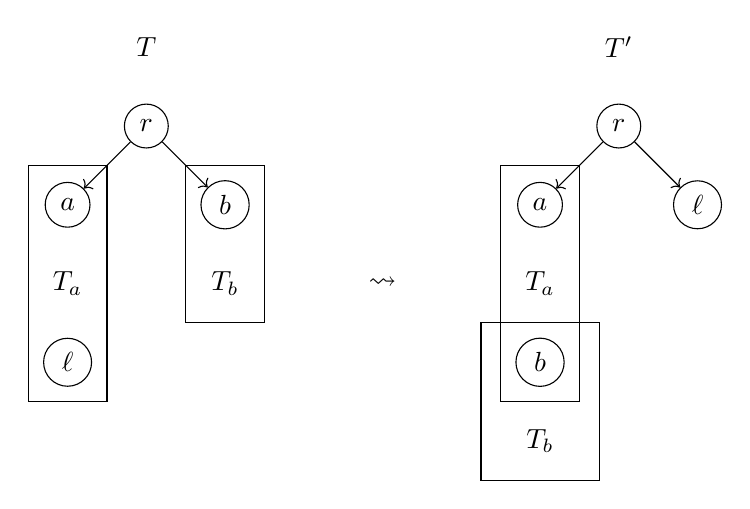
\begin{tikzpicture}
            \begin{scope}[xshift=-3cm]
                \node at (0, 1) {$T$};

                \node[draw, circle] (r) at (0, 0) {$r$};
                
                \node[draw, circle] (a) at (-1, -1) {$a$};
                \draw[->] (r) -- (a);
                \draw (-1.5, -0.5) rectangle +(1, -3);
                \node at (-1, -2) {$T_a$};
                \node[draw, circle] at (-1, -3) {$\ell$};

                \node[draw, circle] (b) at (1, -1) {$b$};
                \draw[->] (r) -- (b);
                \draw (0.5, -0.5) rectangle +(1, -2);
                \node at (1, -2) {$T_b$};
            \end{scope}
            \node at (0, -2) {$\rightsquigarrow$};
            \begin{scope}[xshift=3cm]
                \node at (0, 1) {$T'$};
                \node[draw, circle] (r) at (0, 0) {$r$};
                
                \node[draw, circle] (a) at (-1, -1) {$a$};
                \draw[->] (r) -- (a);
                \draw (-1.5, -0.5) rectangle +(1, -3);
                \node at (-1, -2) {$T_a$};

                \node[draw, circle] (ell) at (1, -1) {$\ell$};
                \draw[->] (r) -- (ell);

                \node[draw, circle] (b) at (-1, -3) {$b$};
                \draw (-1.75, -2.5) rectangle +(1.5, -2);
                \node at (-1, -4) {$T_b$};
            \end{scope}
        \end{tikzpicture}
    \end{center}
    The values of $s(r)$, $s(\ell)$, and $s(v)$ for $v \in V(T_b)$ have not changed.
    However, the values of $s(v)$ for $v \in V(T_a)$ has possibly increased.
    In particular, the value of $s(a)$ has increased by $s(b) - 1 > 0$, since the subtree of $T'$ rooted at $a$ contains all of $T_a$ (except $\ell$), now in addition to all of $T_b$.
    Thus,
    \[
        \sum_{v \in V(T')} s(v) > \sum_{v \in V(T)} s(v).
    \]
    But $T'$ is a full binary tree with $t$ leaves, which contradicts the maximality of $T$'s sum.
    We therefore conclude that either $a$ or $b$ is a leaf, i.e., $r$ has at least one child which is a leaf.
    This completes the induction.
\end{proof}

For a given value of $t$, there is only one possible full rooted binary tree with $t$ leaves satisfying the property that every non-leaf vertex has at least one child which is a leaf.
For example, with $t = 8$ the only possible tree is the following:
\begin{center}
    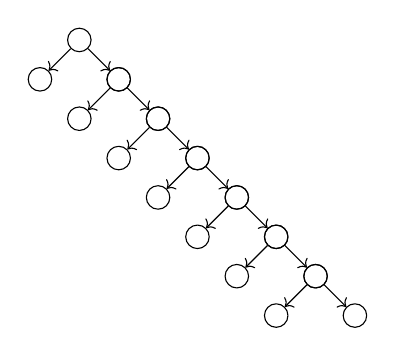
\begin{tikzpicture}[scale=0.5]
        \foreach \t in {0, 1, 2, 3, 4, 5, 6} {
            \node[draw, circle, inner sep=3pt] (r) at (\t, -\t) {};
            \node[draw, circle, inner sep=3pt] (a) at (\t-1, -\t-1) {};
            \node[draw, circle, inner sep=3pt] (b) at (\t+1, -\t-1) {};

            \draw[->] (r) -- (a);
            \draw[->] (r) -- (b);
        }
    \end{tikzpicture}
\end{center}
Then Lemma 2 is actually telling us that any full rooted binary tree with $t$ leaves which maximizes the sum must precisely be the unique such tree satisfying the property that every non-leaf vertex has at least one child which is a leaf.
In other words, there is a unique full rooted binary tree with $t$ leaves which maximizes the sum and, moreover, it is precisely the unique such tree satisfying the property.

For the tree with $8$ leaves, the sum in question is $\sum_{v \in V(T)} s(v) = 71$.


\newpage
\pnum{(c)}

One could argue, using techniques similar to those used in (b), that a tree maximizing this sum must satisfy the property that for every non-leaf vertex, the subtrees rooted at each of its children must have the same number of leaves (possibly $\pm1$ for odd total numbers of leaves).
In which case, there is a unique (for suitable values of $t$) full rooted binary tree maximizing the sum and, moreover, it is precisely the unique such tree satisfying the property.
For $t = 8$, we get the following tree:
\begin{center}
    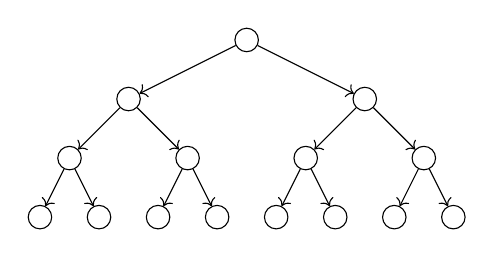
\begin{tikzpicture}[scale=0.75]
        \node[draw, circle, inner sep=3pt] (r) at (0, 0) {};

        \node[draw, circle, inner sep=3pt] (v0) at (-2, -1) {};
        \node[draw, circle, inner sep=3pt] (v1) at (2, -1) {};

        \node[draw, circle, inner sep=3pt] (v00) at (-3, -2) {};
        \node[draw, circle, inner sep=3pt] (v01) at (-1, -2) {};
        \node[draw, circle, inner sep=3pt] (v10) at (1, -2) {};
        \node[draw, circle, inner sep=3pt] (v11) at (3, -2) {};

        \node[draw, circle, inner sep=3pt] (v000) at (-3.5, -3) {};
        \node[draw, circle, inner sep=3pt] (v001) at (-2.5, -3) {};
        \node[draw, circle, inner sep=3pt] (v010) at (-1.5, -3) {};
        \node[draw, circle, inner sep=3pt] (v011) at (-0.5, -3) {};

        \node[draw, circle, inner sep=3pt] (v100) at (0.5, -3) {};
        \node[draw, circle, inner sep=3pt] (v101) at (1.5, -3) {};
        \node[draw, circle, inner sep=3pt] (v110) at (2.5, -3) {};
        \node[draw, circle, inner sep=3pt] (v111) at (3.5, -3) {};


        \draw[->] (r) -- (v0);
        \draw[->] (r) -- (v1);

        \draw[->] (v0) -- (v00);
        \draw[->] (v0) -- (v01);
        \draw[->] (v1) -- (v10);
        \draw[->] (v1) -- (v11);

        \draw[->] (v00) -- (v000);
        \draw[->] (v00) -- (v001);
        \draw[->] (v01) -- (v010);
        \draw[->] (v01) -- (v011);
        \draw[->] (v10) -- (v100);
        \draw[->] (v10) -- (v101);
        \draw[->] (v11) -- (v110);
        \draw[->] (v11) -- (v111);
    \end{tikzpicture}
\end{center}
The sum here is $\sum_{v \in V(T)} p(v) = 12$.

\pnum{(d)}

\begin{proof}
    We perform induction on $t$.

    For the base case, if $t = 1$, then $\ell$ is the only vertex of $T$ so
    \[
        \{u \in V(T) : \ell \in P(u)\} = \emptyset
    \]
    and $t = 1 = 2^{|\emptyset|}$.

    For the inductive step, assume the result holds for any tree with fewer than $t > 1$ leaves.
    Let $r$ be the root vertex of $T$ with children $a$ and $b$.
    Let $T_a$ and $T_b$ be the subtrees rooted at the respective vertices, and denote their numbers of leaves by $t_a$ and $t_b$.
    Notice that $t = t_a + t_b$ with $0 < t_a < t$ and $0 < t_b < t$.
    Without loss of generality, say $\ell$ is a leaf of $T_a$, then the inductive hypothesis gives us
    \[
        t_a \geq 2^{|\{u \in V(T_a) \;:\; \ell \in P(u)\}|}.
    \]
    We now consider two cases: either $\ell \notin P(r)$ or $\ell \in P(r)$.

    In the former case, the only vertices $u \in V(T)$ with $\ell \in P(u)$ are in $T_a$, so
    \[
        \{u \in T(V) : \ell \in P(u)\} = \{u \in V(T_a) : \ell \in P(u)\}.
    \]
    In which case, we deduce
    \[
        t
            \geq t_a
            \geq 2^{|\{u \in V(T_a) \;:\; \ell \in P(u)\}|}
            = 2^{|\{u \in V(T) \;:\; \ell \in P(u)\}|}.
    \]

    In the latter case, $\ell \in P(r)$ by definition requires $s(a) \leq s(b)$.
    Applying Lemma 1, we obtain
    \[
        t_a = \frac{s(a) + 1}{2} \leq \frac{s(b) + 1}{2} = t_b.
    \]
    Moreover,
    \[
        \{u \in T(V) : \ell \in P(u)\} = \{u \in V(T_a) : \ell \in P(u)\} \cup \{r\},
    \]
    so indeed
    \[
        t
            = t_a + t_b
            \geq 2t_a
            \geq 2^{|\{u \in V(T_a) \;:\; \ell \in P(u)\}| + 1}
            = 2^{|\{u \in V(T) \;:\; \ell \in P(u)\}|}.
    \]
    This completes the induction.
\end{proof}


\pnum{(e)}

\begin{proof}
    For $u \in V(T)$ let $\chi_{P(u)}$ be the indicator function of $P(u)$, i.e., for $\ell \in L$
    \[
        \chi_{P(u)}(\ell) = \begin{cases}
            1 &\text{if } \ell \in P(u), \\
            0 &\text{otherwise}.
        \end{cases}
    \]
    We can then write the sum as
    \begin{align*}
        \sum_{u \in V(T)}p(u)
            &= \sum_{u \in V(T)} |P(u)| \\
            &= \sum_{u \in V(T)} \sum_{\ell \in P(u)} 1 \\
            &= \sum_{u \in V(T)} \sum_{\ell \in L} \chi_{P(u)}(\ell) \\
            &= \sum_{\ell \in L} \sum_{u \in V(T)} \chi_{P(u)}(\ell) \\
            &= \sum_{\ell \in L} \sum_{\substack{u \in V(T) \\ \ell \in P(u)}} 1 \\
            &= \sum_{\ell \in L} |\{u \in V(T) : \ell \in P(u)\}|
    \end{align*}
\end{proof}

\pnum{(f)}

\begin{proof}
    The result of (d) can equivalently be written as
    \[
        |\{u \in V(T) : \ell \in P(u)\}| \leq \log t.
    \]
    Combing this with (e) gives
    \[
        \sum_{u \in V(T)} p(u)
            \leq \sum_{\ell \in L} \log t
            = t \log t.
    \]
\end{proof}


\pnum{(g)}

Perform the operations
\[
    \mathsf{Union}(1, 2), \mathsf{Union}(1, 3), \dots, \mathsf{Union}(1, n/2).
\]
This puts the elements $1, 2, \dots, n/2$ into the same component.
Next, perform the operations
\[
    \mathsf{Union}(n/2 + 1, n), \mathsf{Union}(n/2 + 2, n), \dots, \mathsf{Union}(n-1, n).
\]
This puts the elements $n/2 + 1, n/2 + 2, \dots, n$ into the same component.

Lastly, we perform the operation $\mathsf{Union}(1, n)$.
This combines the two components, both of which are $n/2$ (possibly $\pm1$) elements long.
Whichever is shorter is drained and appended to the other, which requires $n/2$ operations.
Hence, the entire process takes $O(n)$ times.

\pnum{(h)}

Suppose we perform the operation $\mathsf{Union}(i, j)$ with corresponding vertex $x$ in the union forest.
In evaluating the operation, we first set $a = \mathsf{Find}(i)$ and $b = \mathsf{Find}(j)$.
After possibly swapping, we may assume $|L[b]| \leq |L[a]|$.
Without loss of generality, say $\mathsf{left}(x)$ corresponds to the $a$ component and $\mathsf{right}(x)$ corresponds to the $b$ component.
Then $L[a]$ is the set of leaves rooted at $\mathsf{left}(x)$ and $L[b]$ is the set of leaves rooted at $\mathsf{right}(x)$.
By assumption $p(\mathsf{left}(x)) \geq p(\mathsf{right}(x))$ which implies $s(\mathsf{left}(x)) \geq s(\mathsf{right}(x))$.
Therefore, $P(x) = L[b]$ and it immediately follows that $p(x) = |L[b]|$.
The time of the union operation is proportional to the size of $L[b]$ (and at least constant time), which is precisely $O(p(x) + 1)$.

\pnum{(i)}

Let $x_1, \dots, x_t$ be the vertices of the union forest corresponding to the $t$ union operations.
Each union operation corresponds to a non-leaf vertex in the union forest.
We are concerned only with the nontrivial trees, i.e., those with more than one vertex, since the trivial trees do not correspond to any actual operations. 
We partition the relevant sub-forest into a number of (nontrivial) full binary trees $T_1, \dots, T_k$.
Since each $T_i$ contains at least one operation vertex $x_j$, we must have $k \leq t$.

Suppose the tree $T_i$ has $t_i$ leaves and $k_i$ non-leaf vertices---the non-leaf vertices corresponding to some of the operations.
Then $T_i$ has $k_i + t_i$ total vertices, and Lemma 1 implies that $t_i = k_i + 1$.
Note that $t = k_1 + \cdots + k_k$.
Then the total number of leaves across the $T_i$ is given by
\[
    \sum_{i=1}^{k} t_i
        = \sum_{i=1}^{k} (k_i + 1)
        = \sum_{i=1}^{k} k_i + \sum_{i=1}^{k} 1
        = t + k
        \leq 2t.
\]
In particular each $t_i \leq 2t$.


Note that $p(\ell) = 0$ for any leaf $\ell$, so (h) tells us that the time needed to perform only the operations contained in $T_i$ is given by
\[
    \sum_{v \in V(T_i)} p(v)
        \leq t_i \log t_i
        \leq t_i \log 2t.
\]
Now since the $T_i$'s partition the $x_j$ operation vertices, the total time for all of the operations is given by
\[
    \sum_{j=1}^{t} p(x_j)
        = \sum_{i=1}^{k} \sum_{v \in V(T_i)} p(v)
        \leq \sum_{i=1}^{k} t_i \log 2t
        \leq 2t \log 2t
        = O(t\log t).
\]




\end{document}